% Requiere TikZ y listings; compilar desde docs/ con el proyecto completo.
\section{Arquitectura de los tres nodos}
\label{sec:arquitectura}
\begingroup
\setlength{\emergencystretch}{2em}

\subsection{Procesos y comunicación con sockets}
El programa \texttt{src/sockets/nodo.py} se ejecuta como tres procesos
identificados por los nombres nodo-A, nodo-B y nodo-C. Cada proceso
escucha en una dirección de loopback y un puerto propio. Al mismo
tiempo, puede enviar mensajes a cualquiera de los otros dos nodos.
La figura~\ref{fig:arquitectura-nodos} representa esta topología
implementada para el registro de eventos de Lamport.

\begin{figure}[htbp]
\centering
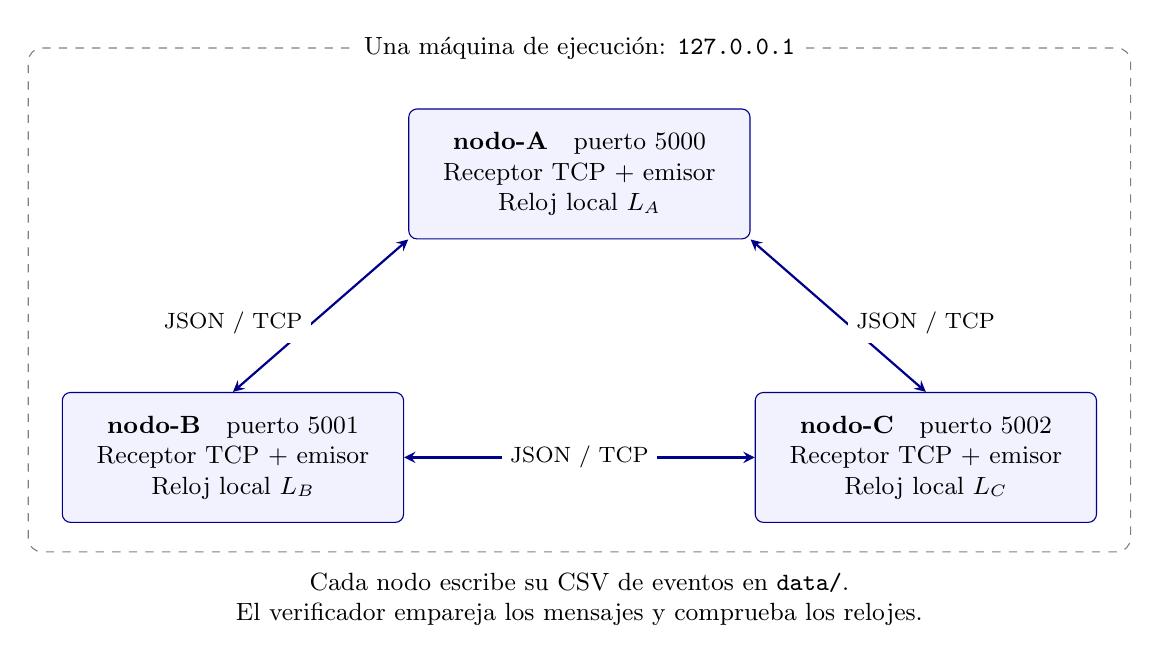
\begin{tikzpicture}[
  servicio/.style={draw=blue!55!black,fill=blue!5,rounded corners=3pt,
    align=center,text width=4.1cm,minimum height=1.65cm,font=\small},
  enlace/.style={<->,>=stealth,thick,draw=blue!55!black},
  etiqueta/.style={fill=white,inner sep=3pt,font=\footnotesize,align=center}
]
\draw[dashed,rounded corners=5pt,gray] (-7,-3.8) rectangle (7,2.6);
\node[font=\small,fill=white] at (0,2.6)
  {Una máquina de ejecución: \texttt{127.0.0.1}};
\node[servicio] (a) at (0,1) {
  \textbf{nodo-A}\quad puerto 5000\\
  Receptor TCP + emisor\\
  Reloj local $L_A$};
\node[servicio] (b) at (-4.4,-2.6) {
  \textbf{nodo-B}\quad puerto 5001\\
  Receptor TCP + emisor\\
  Reloj local $L_B$};
\node[servicio] (c) at (4.4,-2.6) {
  \textbf{nodo-C}\quad puerto 5002\\
  Receptor TCP + emisor\\
  Reloj local $L_C$};
\draw[enlace] (a.south west) -- node[etiqueta,pos=0.55,left]
  {JSON / TCP} (b.north);
\draw[enlace] (a.south east) -- node[etiqueta,pos=0.55,right]
  {JSON / TCP} (c.north);
\draw[enlace] (b.east) -- node[etiqueta] {JSON / TCP} (c.west);
\node[align=center,font=\small] at (0,-4.4) {
  Cada nodo escribe su CSV de eventos en \texttt{data/}.\\
  El verificador empareja los mensajes y comprueba los relojes.};
\end{tikzpicture}

\caption{Tres procesos TCP en localhost. Las flechas dobles representan
la posibilidad de enviar mensajes en ambos sentidos entre cada par.}
\label{fig:arquitectura-nodos}
\end{figure}

Cada nodo mantiene un contador lógico y un candado para coordinar su
actualización entre los hilos de envío y recepción. Un hilo escucha
conexiones entrantes y crea un hilo de atención por conexión.
El emisor elige un destino, incrementa su reloj y envía un JSON
codificado en UTF-8, delimitado por un salto de línea.
TCP proporciona el flujo fiable y ordenado sobre el cual la aplicación
delimita sus mensajes \cite{eddy2022tcp}.

El JSON contiene \texttt{sender}, \texttt{timestamp} y \texttt{message}.
En sockets, \texttt{timestamp} transporta el valor entero del reloj de
Lamport; el identificador de mensaje se incorpora al comienzo de
\texttt{message}, separado del texto por una barra vertical.
Cada proceso guarda el nodo, tipo de evento, reloj, hora real,
identificador y contraparte en su propio CSV.

Este programa registra envíos y recepciones para comprobar el orden
causal. La medición RTT se realizó con los servidores de eco de
\texttt{src/sockets/latencia.py} y \texttt{src/grpc/latencia.py},
que devuelven la solicitud para medir el ciclo completo. No se
confunden esos RTT con la corrida de eventos de Lamport.

\subsection{Contrato de gRPC y Protocol Buffers}
El contrato se define en \texttt{proto/communication.proto} y los
módulos de Python generados están en \texttt{src/grpc/generated/}.
El servicio \texttt{CommunicationService} declara una llamada unaria:
\texttt{ExchangeMessage} recibe una solicitud y devuelve una respuesta.
El listado siguiente se lee directamente del contrato del repositorio.

\lstinputlisting[
  language={},
  morekeywords={syntax,package,service,rpc,returns,message,string,int64},
  literate={í}{{\'i}}1
]{../proto/communication.proto}

Los mensajes \texttt{MessageRequest} y \texttt{MessageResponse}
comparten cuatro campos. \texttt{sender} identifica al emisor y
\texttt{message} lleva el contenido. El campo \texttt{timestamp} se
declara como texto, mientras que \texttt{lamport\_clock} es un entero
de 64 bits destinado al reloj lógico. Al comparar ambos mecanismos,
el reloj que viaja en \texttt{timestamp} de sockets se corresponderá
con \texttt{lamport\_clock} de gRPC. El \texttt{timestamp} textual
contiene una fecha y hora generada por la implementación gRPC.

Protocol Buffers define el esquema de los mensajes y su codificación
binaria \cite{jackson2024streaming}. HTTP/2 aporta los flujos y las
tramas de la conexión utilizada por gRPC \cite{thomson2022http2}.
Los nodos ejecutables de gRPC ya están en \texttt{src/grpc/nodo.py}.
Usan los puertos 50051, 50052 y 50053 para A, B y C, respectivamente,
con la misma topología entre pares. El campo \texttt{timestamp}
contiene la hora física como texto y \texttt{lamport\_clock} el
contador lógico. Las pruebas de latencia tienen servidores de eco
específicos: sockets escucha en el puerto 5000 y gRPC en el 50054.
Estos servidores permiten medir la solicitud y su respuesta.
\endgroup

\subsection{Fragmentos del registro y del acuse}
El nodo TCP actualiza el reloj al recibir el JSON dentro del candado.
El fragmento siguiente se lee del código publicado:
\lstinputlisting[firstline=40,lastline=45]{../src/sockets/nodo.py}

En la versión gRPC actual, la solicitud y su acuse tienen
identificadores separados. Después de registrar la recepción,
el servidor incrementa el reloj para enviar el acuse:
\lstinputlisting[firstline=70,lastline=76]{../src/grpc/nodo.py}

El cliente comprueba el acuse y actualiza su reloj con el valor
devuelto antes de registrar la recepción. Así se cubren los cuatro
eventos de cada solicitud y respuesta:
\lstinputlisting[firstline=108,lastline=109]{../src/grpc/nodo.py}
